\graphicspath{{chapters/images/09/}}

\chapter{Staphylococcus aureus}

\section{Introduction}
\emph{Staphylococcus aureus} is a gram positive (it has a peptidoglican layer into the cell wall) and it is a facultative anaerobe bacterium.
This is very for its epidemiology because it is able to colonize nostrils where there is oxygen, but it is also able to colonize organs that are inside the body.
It is  one of the main players in common food poisoning.
It is also involved in the menstrual toxic shock syndrome.
It plays a key role, also, in other serious disease, like osteomyelitis (infection of the bones) or sepsis (systemic infections).
It is a common skin colonizer and for this reason $25\%$ of the people probably have it, but it is also the cause of very bad skin infection.
The main reason for \emph{S. aureus} to be tricky to treat because of his immune evasion strategies.

\subsection{Immune evasion strategies}
\emph{S. aureus} has two different main strategies that used in order to stop the immune system of the host from getting rid of it.

    \subsubsection{Prevention of the engagement of the host immune system}
    It prevents the engagement of the host immune system, so it is not be recognized by the host immune system.
    That is done by for different classes proteins that are present on the  surface of \emph{S. aureus} able to hide it from the host immune system:

    \begin{multicols}{2}
        \begin{itemize}
            \item Adhesins bind complement factors to inhibit complement activation cascade.
            \item Leukocidins are instead a number of toxins that are selectively killing the adapting immune cells, so killing those immune cells that would be able to kill \emph{S. aureus}.
            \item Immunoglobulin binding proteins bind and immobilize IgGs, so they cannot start the cascade of activation of the immune systems.
            \item Proteases that cleave the immunoglobulin that are responsible for the activation of the host immune system.
        \end{itemize}
    \end{multicols}

    \subsubsection{Overactivation of the non-specific immune system}
    It is able to trigger a lot of inflammation to cytokine release, a non-specific reaction of the body, and also to facilitate invasion of the so-called non-professional phagocytes, the neutrophiles.
    There is the production of autholysins, that facilitate invasion of non-professional phagocytes, and super-antigens, that activate T cells and trigger the cytokine release.
    This could be an advantage to \emph{S. aureus} because when a neutrophiles phagocytes a bacterium or any pathogen can happen that the microbiome is uptaken by the neutrophile, is killed through degranulation and ROS production.
    The neutrophile then undergoes apoptosis and it is removed by macrophages and so there is a resolution of the infection.
    However, \emph{S. aureus} stops the apoptosis of the neutrophile that can uptake it and is able to divide inside it and be screened by the immune system of the host and then, with the leukocidins, it can cause some holes in the neutrophile and in turn the release of its content outside causing an extra inflammation.

\section{Antibiotic resistance in \emph{S. aureus}}
After the discovery in the $1940s$ of penicilin S. Aureus developed quickly the protein penicilinase, becoming resistant to that antibiotic.
Also a few years after the discovery of methicillin, a semisynthetic penicillinase-resistance $\beta$-lactam antibiotic some cases of S. aureus resistant to that antibiotic or MRSA were found in an hospital in the UK and then quickly spread in many countries.

    \subsection{Methicillin-resistant \emph{S. aureus} (MRSA)}
    \emph{S. aureus} is resistant to \emph{beta}-lactam and is also able to acquire other resistances, event to last resource antibiotics, like vancomycin, linezolid, daptomycin.
    Because \emph{S. aureus} is a gram-positive bacterium, the peptidoglycan layer of the cell wall is extremely important for the correct assembly of the cell membrane and the $\beta$-lactam antibiotics have the ability to act as an analog substrate causing an impaired transpeptidation of the peptidoglycan and the creation of a defective cell wall during cell division.

    \begin{multicols}{2}
        \begin{enumerate}
            \item In absence of $\beta$-lactam antibiotics, there is the normal cell-wall biosynthesis.
            \item In presence of $\beta$-lactam antibiotics, the binding of the antibiotic to the PBP active site causes an inability to transpeptidate the peptidoglycan.
                Because of this the peptidoglycan layer of the cell wall cannot be produced and the bacterium dies during cell division.
            \item In presence of the $\beta$-lactam antibiotics, but with mutated PBP (PBP$2$a, or MecA), $\beta$-lactam is not able to bind the modified PBP, the peptidoglycan can be normally transpeptidated and \emph{S. aureus} can produce the cell wall and proliferate.
        \end{enumerate}
    \end{multicols}

    \subsection{Coding of methicillin resistance}
    The resistance to methicillin, but more in general to $\beta$-lactam is encoded on the mobile genetic element staphylococcal chromosome cassette \emph{mec} (SCC\emph{mec}).
    SCC\emph{mec} are mobile genetic elements that are wide spread across staphylococci genome.
    They commonly carries genes that might confer some increased fitness for specific environments.
    This type of mobile genetic elements can be easily integrated into the genome and also can easily excises from it.
    That means that is really easy for a MSSA to integrate the mobile genetic element in case of a strong selective pressure that might be given by the presence of antibiotic.
    When the antibiotic is not more present, it is easy for MSSA to excise the mobile genetic element and return to the basic state of methicillin asset of the \emph{S. aureus}.
    This genetic element is not maintained inside the cell but it is integrated into the it and it is excised and released outside when is no longer needed.

    \subsection{Methicillin-resistant \emph{S. aureus} (MRSA)}
    S. aureus is not well recognized for the problems that it causes.
    There are 80 thousands new patients per year in US that have invasive infections and the mortality rate is at $20\%$.
    Hospitalized patients, immune compromised patients or patients with conditions like cystic fibrosis are very exposed to \emph{S. aureus}.
    This is why, in 2017, the World Health Organization insert \emph{S. aureus} resistant to meticillin and partially resistant to vancomycin or completely as the fifth highest priority bacterium for the research and the development of new antibiotics.
    An article of three years ago estimated about 5 millions deaths associated with bacterial antibiotic resistances (not \emph{S. aureus} only) in $2019$.
    The World Health Organization has estimated that by 2025 there will be 10 millions deaths per years because of antibiotic resistance.

    \subsection{\emph{S.aureus} worldwide}
    There are lot of studies that focused on MRSA or \emph{S. aureus} infections, but the problem is that there are quite biases toward specifically lineages.
    Lineages are specific strains or a group of strains that are known to be particularly hyper-virulent or resistant or affecting a specific population.
    Because of this research is restricted to only a part of the pool of infections that S. Aureus can cause.
    There is a great variability in MRSA that can change epidemiology:

    \begin{multicols}{2}
        \begin{itemize}
            \item $60$s-$70$s. There were lots of hospitals associated infections, so people go to the hospital, get a surgery and get \emph{S. aureus}.
                Also, nowadays \emph{S. aureus} is a key player in post-surgery infections.
            \item $80$s-$90$s. The community start talking about community-associated \emph{S. aureus} infections and methicillin resistance of \emph{S. aureus} because the study starting focusing on the dissemination, also in healthy people.
            \item $2000$s. There was great studies on livestock-associated MRSA.
                Zoonotic infections are pretty relevant, but treatment with antibiotics cause resistances in that community.
                Livestock diseases and resistances are serious consequences.
        \end{itemize}
    \end{multicols}

\section{Whole genome epidemiology, characterization, and phylogenetic reconstruction of \emph{S. aureus} strains in a pediatric hospitals}
The work presented here represent a full pipeline to perform a survey of the general population of S. aureus in a specific place.

\begin{figure}[h]
\centering
\caption{}
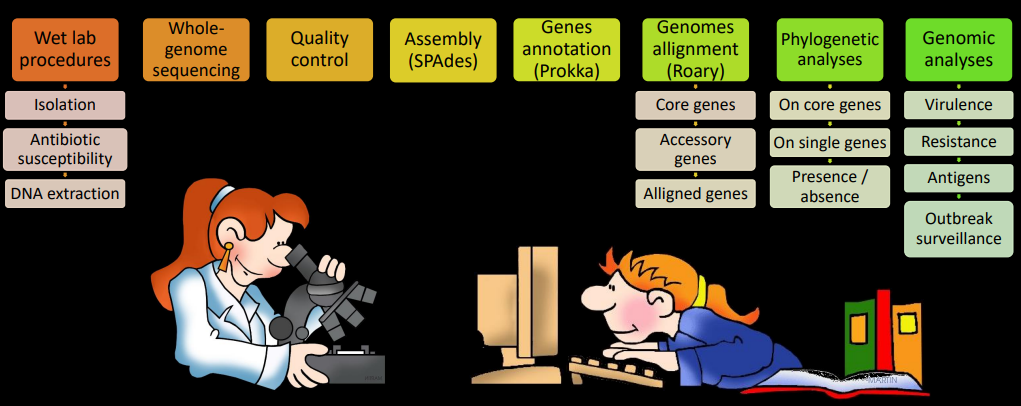
\includegraphics[width=1.0\textwidth]{Workflow.png}
\caption{Wet and dry lab workflow}
\end{figure}

    \subsection{Methods}
    The authors worked with $11$ operative units isolated from each other and they started with $234$ S. aureus isolates performing antibiotic susceptibility test in vitro and whole-genome sequencing.
    After that, they selected 184 of the isolates  with $N50>50k$ to consider only high-quality genomes.
    Patients were not selected on the bases of their status and came from different department of the hospital.
    135 single patients were selected so that all single patients were isolated.
    The genome considered had:

    \begin{multicols}{2}
        \begin{itemize}
            \item Average nr of contigs = $51$ ($12$-$138$)
            \item Average N$50$ = $206$k ($50$k-$970$k)
        \end{itemize}
    \end{multicols}

    Also the samples derived from different tissues like sputum, nasal,  pharyngeal and lesion swabs among the others.

    \subsection{Typing methods}
    Usually the typing of \emph{S. aureus} is based on four different typing methods created for wet-lab work:

    \begin{multicols}{2}
        \begin{enumerate}
            \item Multilocus sequence typing (MLST).
            \item \emph{S. aureus} proteins A (spa).
                It is one of the major determinant of virulence on \emph{S. aureus}.
            \item Staphylococcal cassette chromosome \emph{mec} (SSC\emph{mec}).
                Looked at the presence or absence of it.
            \item Proton-Valentine Leukocydin (PVL).
                Looked at the presence or absence of it.
        \end{enumerate}
    \end{multicols}

        \subsubsection{MLST}
        Multilocus sequence typing consisted in:

        \begin{multicols}{2}
            \begin{enumerate}
                \item Characterizing isolates by sequencing fragments of house-keeping genes.
                \item Each isolate is characterized by its allelic profile at the house keeping loci determining its sequence type (ST).
                \item Based on multilocus enzyme electrophoresis (MLEE).
                    This step is not usually done because of its inefficiency and the high number of PCR required.
                    Allelic profiling is usually much faster since only sequencing and comparison are required.
            \end{enumerate}
        \end{multicols}

        MLST take fragments of house-keeping genes and look at their sequence to assign an allelic profile.
        Looking at each of the $7$ house-keeping genes of S. aureus a sequence of numbers created by the composition of its sequence is compared to a database to determine the lineage of the sample.

        \subsubsection{Spa-typing}
        Spa-typing consists in:

        \begin{multicols}{2}
            \begin{enumerate}
                \item Single locus DNA-sequencing of the repeated region of the Staphylococcus protein gene (spa).
                \item This in turn is used to further discriminate STs.
                \item Repeats are assigned a numerical code and the spa-type is deduced from the order of repeats.
            \end{enumerate}
        \end{multicols}

        The Staphylococcus protein A typing looks at the differences in the repeat sequence internal in the Staphylococcus protein A gene.
        This gene has a part of repeats that can be in different positions.
        The order of the repeats is the determinant of the spa-type.
        To perform this analysis $135$ PCRs were necessary.

        \subsubsection{SCC\emph{mec}}
        During the sequencing of the region containing \emph{mecA} it was found a distinct mobile genetic element named the staphylococcal chromosome cassette \emph{mec} (SCC\emph{mec}).

        \begin{figure}[h]
        \centering
        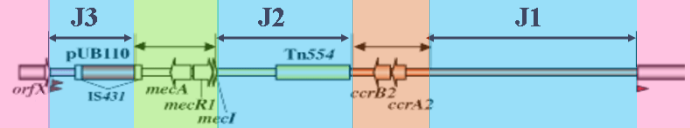
\includegraphics[width=0.6\textwidth]{SCCmec.png}
        \caption{}
        \end{figure}

        The mec gene complex is formed by mecA, mecI and mecR.
        The first is responsible for antibiotic resistance, the second is the inhibitor of the first and the third is the inhibitor of the second.
        While mecA is always present, the other two contribute to the typing of the cassette.
        Another part important for the typing is the cassette chromosome recombinase ccr.
        Moreover there are $3$ joining regions responsible for other resistance that can be used for subtyping.
        There are specific inverted and directed repeats containing the insertion site recognized by the ccr-encoded recombinase.
        There are $11$ types of cassette with different sized and gene content..
        SCCmec perform typing on the mec and ccr gene complez and subtyping on the J region.
        To perform this analysis $675$ PCRs were performed.

        \subsubsection{PVL}
        PVL is a regarded as an important indicator of \emph{S. aureus} virulence.
        The PVL factor is encoded in a prophage that secretes two toxins LukS-PV and LukF-PV.
        It is a good indicator of how invasive an infections can be.
        PVL:

        \begin{multicols}{2}
            \begin{itemize}
                \item Assemble in the membrane of host white blood cells, monocytes, and macrophages.
                \item Form a ring with a central pore through which immune-cell contents leak.
                \item The ring also acts as a superantigen and we have the suppression of adaptive immune response.
            \end{itemize}
        \end{multicols}

        To characterize this gene $135$ PCRs were made.
        In total to get the typing of the community $1890$ PCRs have been performed.

    \subsection{The cohort}
    $1464$ core genes that are present in at least 99$\%$ of the strains and some trees that are quite specific, highly observed through MLST typing.
    A lot of information about sample type, operative unit, PVL presence, SCC\emph{mec} type and presence of virulence genes about the samples.
    To catch virulence genes a list of genes known in literature to cause virulence in S. aureus was compared with the analyzed genoms.
    In the cohort they found:

    \begin{multicols}{2}
    \begin{itemize}
        \item $28$ STs ($14$ CCs)
        \item $41$ \emph{spa}-types
        \item $4$ SCC\emph{mec} types
        \item $27.4\%$ PVL+
    \end{itemize}
    \end{multicols}

    There are $8373$ genes in total that are present in at least 1 isolates.

    \subsection{Co-presence of local, global, animal-associated and hypervirulent clones}

    \begin{figure}[h]
    \centering
    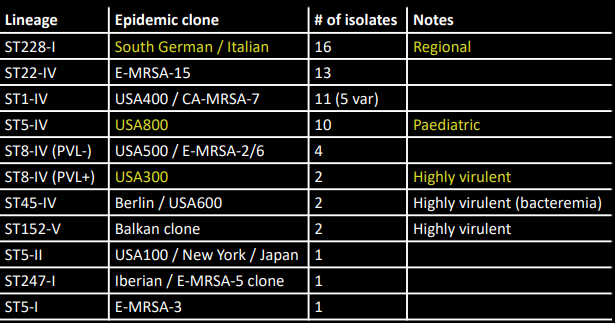
\includegraphics[width=0.6\textwidth]{Highlights.png}
    \caption{}
    \end{figure}

    \begin{multicols}{2}
        \begin{enumerate}
            \item Highly virulent STs:
            \begin{itemize}
                \item USA$300$ ST$8$-SCC\emph{mec}IV PVL+.
                \item ST$239$ HA-MRSA had high transmissibility and quickly develops into bacteria.
                \item ST$45$-SCC\emph{mec}IV causes bacteremia and was an MSSA isolated from infectious diseases.
                \item ST$121$ MSSA obtained from lesion swabs.
                \item ST$152$-SCC\emph{mec}V that caused severe infections.
            \end{itemize}
            \item Livestock-associated MRSA (LA-MRSA), like ST398 and ST97 that causes mastitis, but also found in children not exposed to livestock.
                Which were increased in non at-risk individuals.
            \item They found also the ST$395$ lineage that is very peculiar and it is usually not found in humans.
                It was find in a child that was not at risk.
                It is particularly interesting because he can exchange DNA with the coagulase negative \emph{S. aureus} (CoNS) because it has modified wall teichoic (WTA).
        \end{enumerate}
    \end{multicols}

    \subsection{Genomic signature of chronic versus acute \emph{S. aureus} infections}
    Correlation of specific departments with virulent STs and PVL+:

    \begin{multicols}{2}
        \begin{itemize}
            \item CF and intensive care correlated with PVL + ST$121$
            \item first aid and diseases correlated with PVL
            \item infectious diseases correlated with ST$45$
        \end{itemize}
    \end{multicols}

    Correlation of sample tipes with virulent STs and PVL+:

    \begin{multicols}{2}
        \begin{itemize}
            \item lesion swabs correlated with MSSA, ST$121$ and PVL.
                Here they found virulent and not resistant infections, and that make sense because it is an acute infections.
            \item Lung isolates (bronchoaspiration material + sputum) correlated with ST$128$, PVL and MSSA.
        \end{itemize}
    \end{multicols}

    They observed that chronic infections are usually less virulent, while normally acute infections are more virulent.

    \subsection{Variability in SSC\emph{mec} cassettes}
    They took cassettes and they performed genomic analysis to specifically check the genes that are present.
    When focusing on a specific part of the genome, presence or absence of genes and their functions can be analysed.
    They found two cassettes harboring extra genes that were resistant at antibiotics (kanamycin, bleomycin and trimethoprim).

    \subsection{Diversity of virulence factors and antigens}
    Specific class of genes can be considered, like immune evasion genes.
    Some immune invasion genes are present in almost all of the isolates.
    The resistant to vancomycin is never present.
    But is present the resistant to penicillin.
    There is only one sample (first aid) positive for Edin (epidermal cell differentiation inhibitor) that causes translocation into the bloodstream.
    One USA300 isolate positive for the arginine catabolic mobile element (ACME) and that increased the pathogenicity of the strain.
    There was an higher prevalence of:

    \begin{multicols}{2}
        \begin{itemize}
            \item resistance genes in chronic infections.
            \item virulence genes in acute infections.
        \end{itemize}
    \end{multicols}

    Toxins primarily responsible for \emph{S. aureus} skin manifestations (Eta and Etb) were strongly associated with ST$121$ and lesions.
    Staphylococcal enterotoxins are present in infections department, but are not also present in CF and intensive care departments.

    \subsection{Virulence factors with available vaccines targets}
    There are no vaccine approved now for \emph{S. aureus}.
    They took a list of genes that encode for the target of these vaccines and they checked for the prevalence in the community of isolates and also the presence of SNPs or deletions.
    There are different strategies for the development of vaccines:

    \begin{multicols}{2}
        \begin{enumerate}
            \item highly prevalent genes, but with an high degree of variability/indels.
            \item most virulent or lethal infections.
            \item non-virulence genes, more prevalent and conserved than virulence ones.
        \end{enumerate}
    \end{multicols}

    They mentioned antigens are part of the formulation of putative vaccines tested in published clinical trial, with only a few of them getting favourable results and no approved vaccine to date.

\subsection{Phylogenetic of specific STs highlights the aggressive spread of a novel independently acquired ST$1$ clone}
They investigated the hypothesis that some of the prevalent STs could be hospital-associated clones:

\begin{multicols}{2}
    \begin{enumerate}
        \item isolates sharing the same ST, SCC\emph{mec}, and \emph{spa} types, were not monophyletic subtrees when considering external genomes for the same STs.
            There is and independent acquisition of the clones and there is no evidence of transmission in the hospital.
        \item two ST$121$ MSSA isolates from two patients in the same time window were found to be almost identical.
        \item all but two isolates belonged to the same sub-lineage, typed as SCC\emph{mec}IV t127 PVL-.
    \end{enumerate}
\end{multicols}

It was used a Bayesian phylogenetic modelling approach integrating in the analysis all the ST1 reference genomes publicly available and the two ST$1$ SCC\emph{mec}V:

\begin{multicols}{2}
    \begin{enumerate}
        \item Meyer's clone emerged $6$ to $28$ years ago as a specific branch of the ST$1$ tree ($26$-$160$ years old).
        \item An isolate obtained in a recent study investigating the spread of a ST$1$ SCC\emph{mec}IV t$127$ clone in Irish hospitals and carrying a virulence and resistance profile very close to the one of our cohort (differences in gene presence: $2$/$79$ and $0$/$18$ respectively) is phylogenetically  rooted inside the Meyer's cluster.
    \end{enumerate}
\end{multicols}

ST$1$ SCC\emph{mec}IV t$127$ is not specific of the Meyer's hospital, but might represent a newly arising community clone that is now spreading in the nosocomial environment of different countries.

\subsection{Conclusions}
With a whole genome sequencing approach we can:

\begin{multicols}{2}
    \begin{enumerate}
        \item Type and phylogenetically reconstruct a large \emph{S. aureus} cohort.
        \begin{itemize}
            \item Observe emerging / unexpected clones.
            \item Spot potential outbreaks.
        \end{itemize}
        \item Test for antibiotic resistances and virulence factors.
        \item Discover variants in genes of interest or of unknown relevant genes.
        \item Track strain transmission among patients.
    \end{enumerate}
\end{multicols}
